% \begin{multicols}{2}

\section{Evaluation}

\subsection{Cross Validations}\label{SECTION: CROSS_VALIDATION}
The hardware used in following sections is Intel i5-12450H CPU 
with 16 GB DDR5 2133MHz memory and 
NVDIA GeForce 4050 GPU with 6GB GDDR5 memory.

In general, $k$-fold cross validation is an approach for tuning models to select 
hyperparameters from given value lists. 
However, cross validation is a high computational expensive approach for 
tuning hyperparameters. 
Without fine tuning to the hyperparameters of feature engineering to 
dataset ($q$ step ahead, $n$ stamps prediction, $d$ sample cycility),
but exclusively for regression models, hyperparameters are $C$, $p$ 
and for LSTM models number of units 
which will be discussed later. 
\paragraph{Strategy}
As mentioned, validating in a wide range of values could be computational 
expensive. 
Thus, the models Lasso and Ridge will be validated on 
$C = \left[ 10^{-3}, 10^{-2}, 1, 10,100,1000 \right]$
and $p = \left[ 1, 2\right]$. 
The LSTM Models will be evaluated with 
number of units in candidates $[1, 50, 100, 1000]$. 
Furthermore, the full data set of trainable data could be still large to 
apply validations at this circumstance where 
totally $5\times 2\times 6=60$ regression models will be evaluated at least.
In order to solving this, the strategy is compromising between 
the precisions of validations 
and the computation demands. 
More specifically, in cross validation process, the training data are only 
a part of pre-pandemic period which is from 2018-08-01 to 2020-10-31. 
The details of training is using Adam optimizer at learning rate $10^{-3}$, and 
$10$ epochs, and the batch size is $32$.
\subsection{Recommendations}
\paragraph{Recommendation of $C$, $p$}

The results are shown in the \ref{FIGURES: Lasso, Ridge, Cross Validation}
and \ref{TABLE: MSE of Ridge and Lasso Regression Models on 5-fold cross validation }
From the results of $5$-fold cross validation for $C$ and $p$ on Ridge and Lasso regression 
models shown in  
\ref{FIGURES: Lasso, Ridge, Cross Validation}. 
It is clear that Lasso and Ridge models have approximately identical 
performance with non-polynomial featured $(p=1)$ data when penalty 
value $C = 1$, $10$, $0.01$ and up to $1000$.  
Thus the recommendation of hyperparameter $p$ is $1$
for computation resources saving. 
\begin{figure}[H]
    \centering
    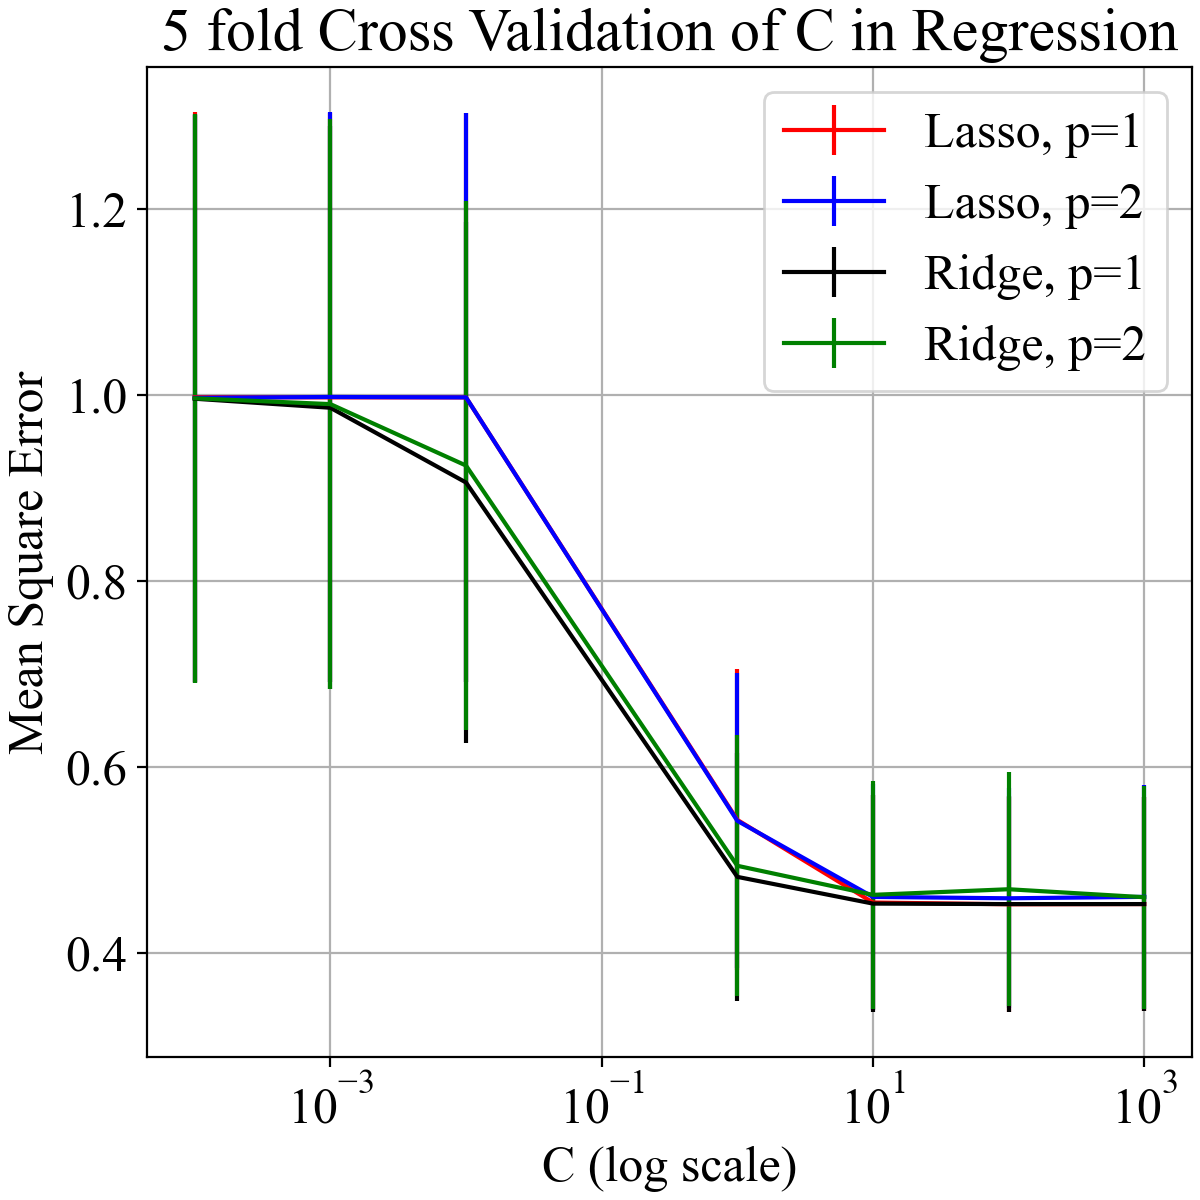
\includegraphics[width=0.4\textwidth]{chap/fig1.png}
    \caption{
        \footnotesize
        MSE of Regression Models $(p=1)$ in
        $5$-fold cross validation
        } % 表格标题
    \label{FIGURES: Lasso, Ridge, Cross Validation}
\end{figure}
However, as the \ref{TABLE: MSE of Ridge and Lasso Regression Models on 5-fold cross validation } shows the mean square error (MSE) of Ridge regression models $(p=1)$
with such various penalty values have same performance as Lasso models. 
Overall, the information of $5$-fold cross validation on Lasso and Ridge models 
does not capable to give a convinced recommendation of hyperparameter $C$.
\begin{table}[H]
    \footnotesize
    \centering
        \caption{
            \footnotesize
        MSE of Regression Models $(p=1)$ in
        $5$-fold cross validation
        } % 表格标题
    \begin{tabular}{ccccc} % 5列,全部居中对齐
        \toprule % 顶线
        $C$ & $1$ & $10$ & $100$ & $1000$ \\ % 表头
        \midrule % 中线
        Ridge & 0.48195 & 0.45320 & 0.45266 & 0.45269 \\ % 第一行数据
        Lasso & 0.54323 & 0.45435 & 0.45247 & 0.45269 \\ % 第二行数据
        \bottomrule % 底线
    \end{tabular}
    \label{TABLE: 
        MSE of Ridge and Lasso 
        Regression Models on 
        5-fold cross validation    
    } % 用于引用表格的标签
\end{table}

\paragraph{Recommendation of units number}
In the case that regression models have approximately identical performance,
the additional LSTM models with $[1, 50, 100, 1000]$ units will be evaluated 
using the strategy in section \ref{SECTION: CROSS_VALIDATION}.
The results of MSE are shown in the \ref{FIGURES: LSTM, Ridge, Cross Validation},
as well as the recommended Ridge Model with 1-polynomial featured data.

With results from the regression models (treated as baseline models),
in the \ref{FIGURES: LSTM, Ridge, Cross Validation}, 
it is clear that LSTM models have better performance comparing 
to the fine tuned Ridge and Lasso models at the beginning ($1$ unit).
\begin{figure}[H]
    \centering
    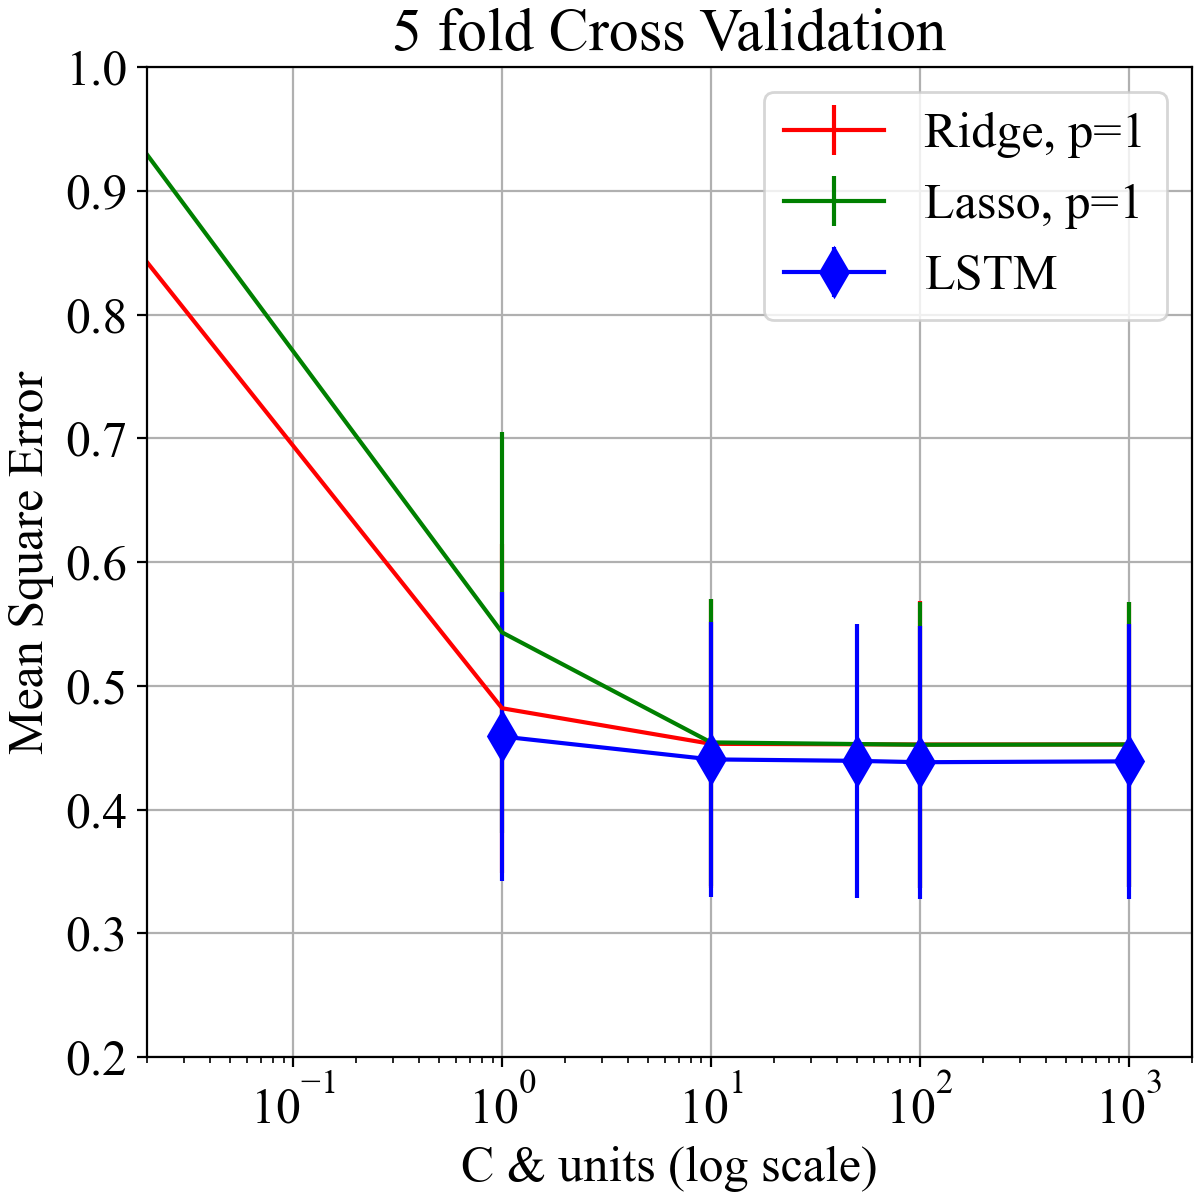
\includegraphics[width=0.4\textwidth]{chap/fig2.png}
    \caption{
        \footnotesize 
        MSE of Regression Models $(p=1)$ in
        $5$-fold cross validation
        } % 表格标题
    \label{FIGURES: LSTM, Ridge, Cross Validation}
\end{figure}
The performance of LSTM model gets to bottleneck as it has around 1000 units 
(due to the limits of hardware, the LSTM which has more units are not capable 
to evaluate). 
\begin{table}[H]
    \footnotesize
    \centering
        \caption{
            \footnotesize
            LSTM RNN model $5$-fold cross validation
        } % 表格标题
    \begin{tabular}{ccccc} % 5列,全部居中对齐
        \toprule % 顶线
        units & $1$ & $10$ & $100$ & $1000$ \\ % 表头
        \midrule % 中线
        LSTM & 0.48195 & 0.45320 & 0.45266 & 0.45269 \\ % 第一行数据
        \bottomrule % 底线
    \end{tabular}
    \label{TABLE: LSTM CROSS VALIDATION   
    } % 用于引用表格的标签
\end{table}
Comparatively, choosing 100 as the number of units is a balance between 
computational cost and performance gained. 

\section{Training LSTM Model}
Considering the recommendations of hyperparameter and 
comparison between regression models and LSTM RNN, the LSTM RNN model 
with a 100 units LSTM layer and a dense layer makes the predictions.
\subsection{Training Settings}
In this case, use the LSTM model with same architecture applied in 
cross validations which is one LSTM layer and one dense layer (prediction layer).
Choosing the training epoch as maximum 100 epoch to ensure the model
sufficiently learned the trends in the given data (pre-pandemic period).
Besides that, in oder to prevent over-fitting, the training strategy includes 
early stopping which means the training process will stop as the metrics of 
fitting process satisfies criterion of tolerance. 

The optimizer of fitting is Adam optimizer same as which applied in validation, 
using the default learning rate setting $(10^{-3})$. 
The batch size is $32$ and 
the tolerance of early stopping is $10^{-4}$,
the patience is $10$ epochs, and it is monitored by validation mean square error 
(mse). 
\begin{figure}[H]
    \centering
    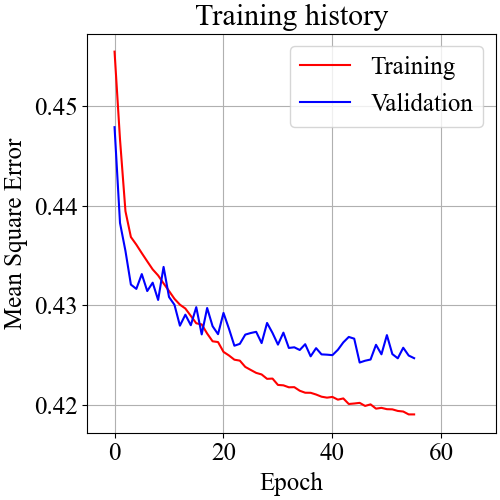
\includegraphics[width=0.35\textwidth]{chap/fig3.png}
    \caption{
        \footnotesize
        Training history of LSTM RNN model on pre-pandemic dataset with 
        100 epochs(stopped at 63th), 32 batch size and Adam optimizer.}
    \label{FIG: Training history of LSTM RNN model on pre-pandemic dataset with 
    50 epochs, 32 batch size and Adam optimizer.}
\end{figure}
\subsection{Results \& Discussion}
The training process early stopped at $56$th epoch iteration where the training 
mse minimized to $0.4202$ and the validation mse is $0.4263$. 
The figure 
\ref{FIG: Training history of LSTM RNN model on 
pre-pandemic dataset with 50 epochs, 32 batch size and Adam optimizer.}
demonstrates that the validation mse did not increase but 
entered the plateau around $40$.
In addition, the mse on testing dataset are $0.4396$ which is close to the validation 
mse. It means that the model learned the general trends behind the given data files.
Therefore, the prediction of the this model could be relatively trustable.